\section{Canberra MRT Station: A Semi-open Waiting-area Case}
\label{sec:rail}

\subsection{Site evidence and the modeled waiting area}

We select Canberra MRT station in Singapore for Requirement 2(b). RSP describes an elevated, two-storey station with a site area of $9,128\,\mathrm{m^2}$ \cite{canberra-rsp}. LTA identifies platform planting, daylight-admitting glazing and rain-protective louvers that allow natural ventilation \cite{canberra-lta}. The design question is which device types, quantities and locations can meet passenger cooling and coverage requirements with the least electricity. We evaluate candidate installations of A, B and C in this shaded, humid, semi-open setting; their deployment is hypothetical.

\begin{figure}[!ht]
\centering
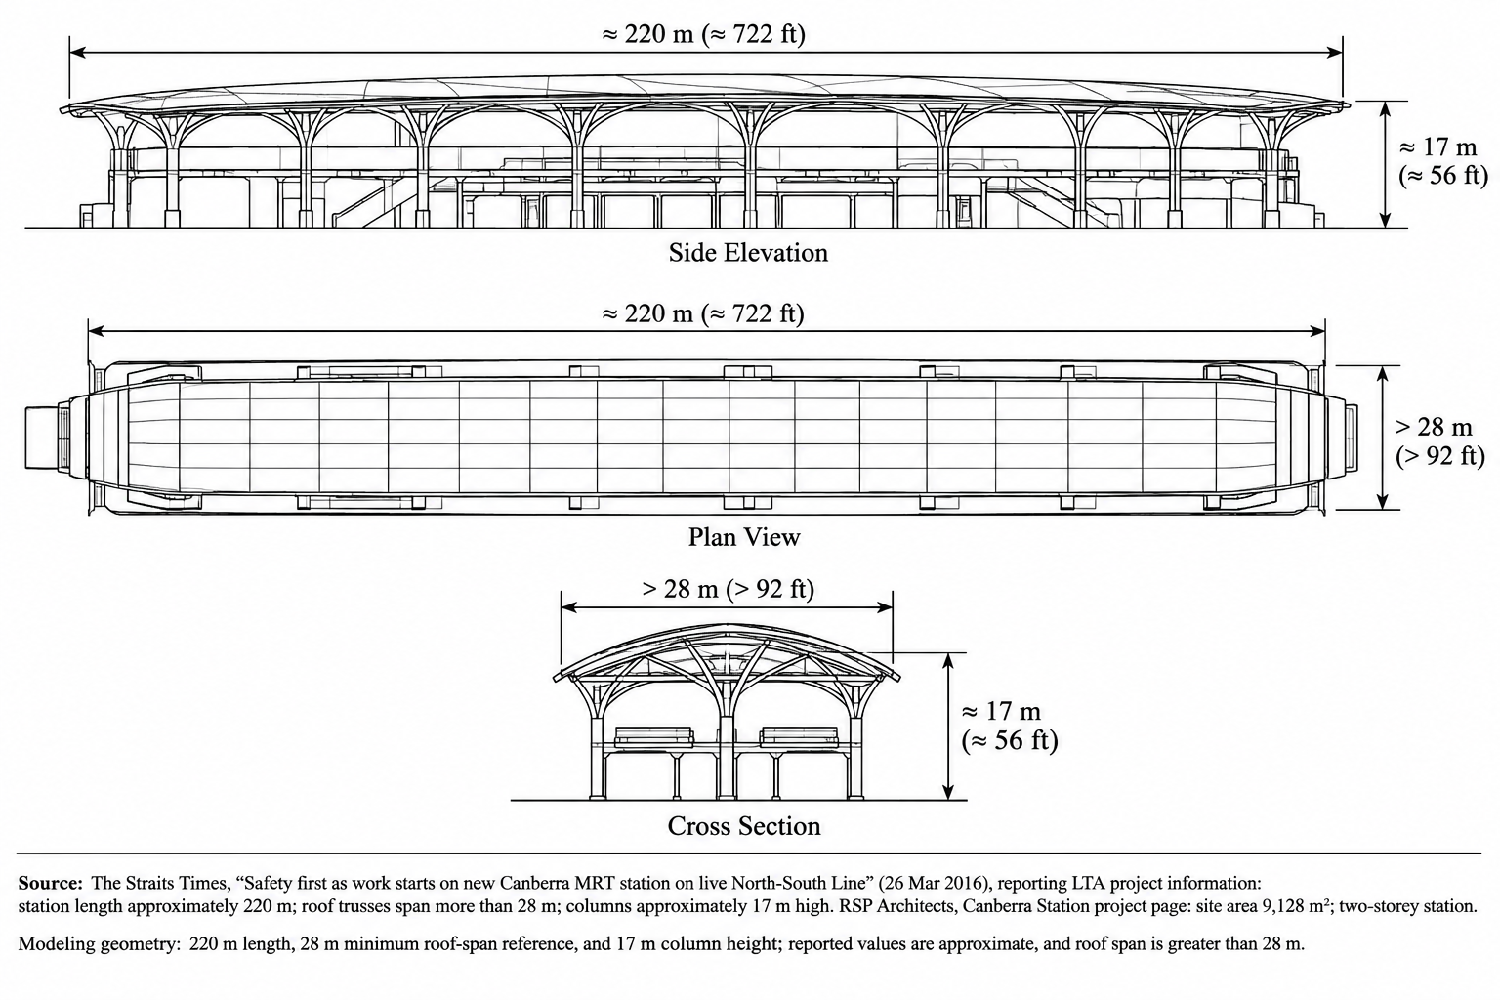
\includegraphics[width=0.84\linewidth]{figures/13_canberra_station.pdf}
\caption{User-supplied Canberra station schematic, retained as a separate PDF. Approximate structural dimensions are contextual references; the drawing is not an as-built survey or a map of the calculation zones. Sources identified in the drawing are listed in \cite{canberra-dimensions,canberra-rsp}.}
\label{fig:canberra}
\end{figure}

\noindent\textbf{Modeled occupied area.} The schematic labels approximately 220 m length, roof span over 28 m and roughly 17 m columns. Roof span and column height are not occupied width or platform clearance. We assume aggregate waiting width $b=6$ m, usable fraction $\alpha=0.8$ and effective background-air height 4 m:
\begin{equation}
 A_{\mathrm{occ}}=\alpha Lb=1056\,\mathrm{m^2}.
\label{eq:canberra-area}
\end{equation}
Three equal aggregate zones, access/core/edge, each have $352\,\mathrm{m^2}$ and $1408\,\mathrm{m^3}$. They represent contrasting exposure conditions, not surveyed compartments. Neither occupied area nor effective height is inferred directly from site area or column dimensions.

\subsection{What changes from the bus model, and why}

The service objective, device response, local mixing operator, SET and energy denominator remain unchanged. What changes is the background state supplying each device. The bus uses a prescribed outdoor reservoir; the station solves Eq.~\eqref{eq:common-balance} with time-varying people, exchange and surface feedback. Local delivered air is then computed using the same Eq.~\eqref{eq:mixing}. This makes the extension traceable at both the physical and service levels.

\begin{table}[!ht]
\centering\small
\caption{Retained modules, released approximations, and their consequences.}
\label{tab:rail-changes}
\begin{tabularx}{\linewidth}{@{}>{\raggedright\arraybackslash}p{0.24\linewidth}XX@{}}
\toprule
Module & Bus simplification & Rail extension and purpose\\
\midrule
Device and local delivery & Fixed outdoor inlet; steady entrainment; local electric heat neglected. & Evolving background inlet; same mixing balance with supply heat, to distinguish local relief from background response.\\
Background heat/moisture & Outdoor reservoir is prescribed. & Solve storage and interzone exchange to capture humidity feedback and time lag.\\
Surfaces & Fixed shaded radiant environment. & Solve effective surface storage and radiative influence.\\
Response and service & SET, signed relief, people-time weighting and all-device energy. & Retain all four; vary counts and locations and assess coverage.\\
\bottomrule
\end{tabularx}
\end{table}

The assumed base exchange of $4$--$10$ h$^{-1}$ gives an air replacement time $(3600/ACH)\,\mathrm{s}=6$--$15$ min, comparable to the assumed 15-min passenger cycle. This supports resolving background dynamics in this scenario; station size alone would not justify it. The local mixing region is treated as having negligible storage only if $\tau_\ell=M_\ell/(\dot m_k+\dot m_e)$ is small relative to the 120-s arrival disturbance. $M_\ell$ is the air held in the local jet core, not footprint area multiplied by the platform height. Its unmeasured residence time is a limitation of this closure.

\subsection{Coupled heat, moisture, and surface balances}

Following the control-volume structure of building heat and moisture balances \cite{epzone}, let each zone store moist-air enthalpy $h_z$ (J/kg dry air), humidity ratio $w_z$ (kg/kg dry air), and an effective roof/wall inner-surface temperature $T_{m,z}$. The background air is well mixed within each aggregate zone; the embedded local delivery regions are evaluated separately with negligible air storage. Background dry-air mass is approximated as constant, $M_z=\rho_{da,o}V_z$, with outdoor reference density. Using the occupied-zone volume for background storage neglects the smaller local jet hold-up. This is a reduced model, not an EnergyPlus or CFD simulation.

Define the exchange operator, for either $x=h$ or $w$, as
\begin{equation}
 \mathcal L_z(x)=\dot m_{0z}(x_o-x_z)+\sum_{j\ne z}\dot m_{zj}(x_j-x_z),
 \qquad \dot m_{0z}=M_z\lambda_z/3600.
\label{eq:rail-exchange}
\end{equation}
Here $\lambda_z$ is the assumed outdoor air-change rate in h$^{-1}$. Each exchange represents equal entering and leaving dry-air flow; adjacent-zone rates satisfy $\dot m_{zj}=\dot m_{jz}$. Wind, buoyancy and opening geometry can affect outdoor exchange \cite{ventilation}; a prescribed train-cycle pulse tests that uncertainty without claiming a station-specific piston-flow law.

With $x_{zk}$ devices of type $k$ in zone $z$, unit circulation $\dot m_k$ (kg dry air/s), and time in seconds, our balances are
\begin{align}
 M_z\dot h_z={}&\mathcal L_z(h)+H_{ma,z}(T_{m,z}-T_z)
 +n_zq_c+n_zg h_v(T_z)+P_z
 +\sum_k x_{zk}\dot m_k(h_{e,zk}-h_z),\label{eq:rail-enthalpy}\\
 M_z\dot w_z={}&\mathcal L_z(w)+n_zg+
 \sum_k x_{zk}\dot m_k(w_{e,zk}-w_z),\label{eq:rail-moisture}\\
 C_{m,z}\dot T_{m,z}={}&H_{mo,z}(T_o-T_{m,z})+Q_{\mathrm{sol},z}
 +n_zq_r-H_{ma,z}(T_{m,z}-T_z).\label{eq:rail-surface}
\end{align}
The per-person inputs are convective heat $q_c$, radiative heat $q_r$, and water-vapor generation $g$. Vapor enters with $h_v(T)=2501000+1860T$ J/kg; no additional latent-heat term is added. With $P_k=1000p_k$ W per unit, total device power is $P_z=\sum_k x_{zk}P_k$ (W). This power ultimately dissipates within the modeled zone. Its division between supply air and background affects local exposure but not total input. Pump power is already included in the device total. Conductances $H$ have units W/K, surface capacity $C_m$ has units J/K, and $Q_{\mathrm{sol}}$ is an effective absorbed envelope load. The opposite signs of the air--surface term conserve internal energy.

Air temperature is recovered from $T_z=(h_z-2501000w_z)/(1006+1860w_z)$. A shaded longwave approximation for the surface contribution to comfort \cite{thermalcomfort} gives
\begin{equation}
 T_{r,z}=\left[F_z(T_{m,z}+273.15)^4+(1-F_z)(T_{r,o}+273.15)^4\right]^{1/4}-273.15.
\label{eq:rail-mrt}
\end{equation}
$F_z$ is an assumed effective view fraction; the example sets external radiant temperature $T_{r,o}=T_o$, while keeping it a separate input. Direct sun on passengers and detailed radiative asymmetry are excluded.

\noindent\textbf{The retained device module.} Evaluate Eq.~\eqref{eq:outlet} using the current background inlet. For A, the unheated circulation outlet equals the background, so its circulation has no net bulk enthalpy or water source. For B/C, $h_{e,zk}\simeq h_z$ while $w_{e,zk}>w_z$ when evaporation occurs. Increasing background moisture reduces subsequent wet-bulb depression. Here the subscript $e$ denotes the unheated outlet, the state labeled $o,s$ in Eqs.~\eqref{eq:outlet}--\eqref{eq:enthalpy}; it does not denote outdoor air. Device electricity remains a separate positive heat source in Eq.~\eqref{eq:rail-enthalpy}.

\subsection{Local delivery without double-counting heat or water}

For each covered subgroup, apply Eqs.~\eqref{eq:supply-heat}--\eqref{eq:mixing} with background $b=z$. We distinguish the treated-stream fraction $\beta_{zk}$ from the passenger coverage fraction $c_{zk}$ defined below. The supply flow draws from the background, entrains additional background air, and returns the mixed air to that same zone. For finite entrainment ($\beta>0$),
\begin{align}
 (\dot m_k+\dot m_e)(h_{\ell,zk}-h_z)+(1-\chi)P_k
 &=\dot m_k(h_{e,zk}-h_z)+P_k,\\
 (\dot m_k+\dot m_e)(w_{\ell,zk}-w_z)
 &=\dot m_k(w_{e,zk}-w_z).
\label{eq:return-closure}
\end{align}
Thus the return flow gives exactly the existing background source. The local state improves the exposure calculation without adding evaporation or electrical heat a second time. People outside direct footprints experience the background state; those inside experience the mixed supply state. Both experience the zone radiant environment. Prescribed air speeds remain a separate approximation; no momentum or detailed jet trajectory is solved.

We set $\beta=0.5$ for each type as an explicit equal-entrainment scenario and use unit circulation flows $0.6/0.6/1.2$ kg dry air/s for A/B/C. These are assumptions, not manufacturer data. The nominal $\chi=1$ puts all electrical dissipation into the air before it reaches passengers, a conservative supply-heating case. The sensitivity analysis varies $\beta$ and $\chi$, and separately varies A's newly assumed circulation flow. The case $\beta=0$ is an infinite-dilution scalar limit that exactly recovers the previous shared-background exposure; it retains the prescribed local speeds and is a diagnostic limit, not a measured finite-flow state.

\noindent\textbf{Recovery of the bus model.} Hold the background at outdoor $h_a,w_a$, prescribe the bus radiant environment, speeds and occupancies, neglect local electrical heating ($\chi=0$), and use the bus $\beta$ values. The same device and delivery functions then give the bus temperatures, humidities, SET and service exactly. Fixing the background corresponds to an outdoor-reservoir approximation to Eq.~\eqref{eq:common-balance}; merely setting time derivatives to zero would not impose it. This distinction makes the reduction physically explicit.

\subsection{Equipment selection, allocation, and coverage}

Here $s$ indexes an installation and $k$ a device type. Let $x_{zk}\in\mathbb Z_{\ge0}$ be the number of devices of type $k\in\{A,B,C\}$ in zone $z$. A $3\times3$ count matrix specifies a candidate installation, allowing quantities and device types to vary by zone. Each candidate is evaluated through the resulting shared thermal environment: all operating units contribute heat and electricity, and evaporative units also contribute moisture.

We use assumed, non-overlapping service footprints $a_A=20$, $a_B=30$ and $a_C=40\,\mathrm{m^2}$ per unit. These are comparison inputs, not manufacturer coverage ratings. For uniform passenger density within a zone, define
\begin{equation}
 c_{zk}=\frac{x_{zk}a_k}{A_z},\qquad
 c_{z0}=1-\sum_k c_{zk}\ge0,\qquad \sum_kx_{zk}a_k\le A_z.
\label{eq:coverage}
\end{equation}
The uncovered fraction experiences local speed $v_0$; each covered subgroup experiences its device-specific speed $v_{zk}$. We average \emph{discomfort}, not velocities or device efficiencies:
\begin{equation}
 \overline D_{s,z}(t)=c_{z0}D[\Theta(T_z,T_{r,z},v_0,\phi_z)]
 +\sum_k c_{zk}D[\Theta(T_{\ell,zk},T_{r,z},v_{zk},\phi_{\ell,zk})].
\label{eq:mixed-discomfort}
\end{equation}
The subgroups share radiant conditions but can differ in air temperature, humidity and speed. An uncovered passenger can still experience indirect background cooling or humidification. Coverage denotes direct delivery, not a boundary of all thermal influence. Separate, non-overlapping footprints approximate distributed equipment; co-located jets, overlap and series operation require additional airflow modeling.

\subsection{Canberra scenario and comparable deployment tests}

We assume $33\,^{\circ}\mathrm C$ and $70\%$ outdoor RH for a hot, humid Canberra scenario. Singapore's weather service describes typical daytime maxima of $31$--$33\,^{\circ}\mathrm C$ and high humidity, with rain-free afternoon RH around $60\%$ \cite{singapore-climate}. Our pair is a scenario, not a simultaneous observation at the station. SET retains $1.2$ met, $0.5$ clo, and the common $26\,^{\circ}\mathrm C$ reference.

\begin{table}[!ht]
\centering\small
\caption{Station-scale scenario: operating assumptions, with powers and outlet caps interpreted from the problem.}
\label{tab:rail-inputs}
\begin{tabularx}{\linewidth}{@{}>{\raggedright\arraybackslash}p{0.27\linewidth}>{\raggedright\arraybackslash}X@{}}
\toprule
Input & Assumed value and interpretation\\
\midrule
People and train cycle & An assumed 15-min stress-test cycle, not the actual timetable. Zone counts rise from $(26.4,44,17.6)$ to $(88,198,66)$, then reset; fractional values represent mean counts.\\
Outdoor and zone exchange & Base ACH $(8,4,10)$ h$^{-1}$, plus $(8,4,12)$ in the last 2 min; adjacent-zone exchange $0.88$ kg dry air/s.\\
Surface response, per zone & $C_m=17.6$ MJ/K; $H_{ma}=880$, $H_{mo}=1760$ W/K; absorbed load $3520$ W; view fractions $(0.55,0.85,0.55)$.\\
Human sources & Convection $45$ W, radiation $30$ W, vapor $45/(2.45\times10^6)$ kg/s per person.\\
Device powers and flows & $p_{A/B/C}=0.25/1.2/2.5$ kW; circulation $0.60/0.60/1.20$ kg dry air/s per unit. B/C use $\varepsilon=0.70$ and $5/8\,^{\circ}\mathrm C$ outlet-drop caps. Local $\beta=0.5$, $\chi=1$.\\
Speeds at covered locations & A $(0.60,1.00,0.50)$, B $(0.50,0.80,0.45)$, C $(0.75,1.00,0.60)$ m/s; uncovered locations $0.20$ m/s.\\
\bottomrule
\end{tabularx}
\end{table}

The same occupied area, thermal properties, load densities and passenger schedule are used for every candidate. This holds demand constant while equipment quantities and allocation change. The architectural sources establish the venue context; the assumed operating conditions and coverage parameters define the numerical comparison.

We first compare six benchmark configurations at the same direct-service footprint: $240\,\mathrm{m^2}$ per zone, or $68.2\%$ of the assumed occupied area. Per-zone counts $(x_A,x_B,x_C)$ are $(12,0,0)$, $(0,8,0)$, $(0,0,6)$, $(6,4,0)$, $(6,0,3)$ and $(3,2,3)$. Whole-station totals are respectively 36, 24, 18, 30, 27 and 24 units. Device-count sweeps then quantify the energy needed for wider coverage, and a fixed-inventory redistribution test isolates the effect of allocation. Together these comparisons address type, quantity and placement.

A prescribed two-hour uncooled warm-up gives all candidates the same initial air and surface states. Each then runs for two hours alongside a no-device trajectory with identical weather, people and exchange. This specifies common prior history without claiming periodic steady state; no free initial stored cooling is credited. Electricity covers all cooling devices, not the whole station bill; benefits after the horizon are excluded.

\subsection{Comparing service, coverage, and electricity}

Retain signed relief against the matched baseline, now using the coverage-weighted discomfort:
\begin{align}
 U_s&=\frac1{3600}\int_0^{7200}\sum_z n_z(t)[D_{0,z}(t)-\overline D_{s,z}(t)]\,dt,\\
 E_s&=\frac1{3600}\int_0^{7200}\sum_{z,k}x_{zk}p_k\,dt,
 \qquad \eta_s=U_s/E_s.
\label{eq:rail-efficiency}
\end{align}
With $t$ in seconds and $p_k$ in kW, the factors $1/3600$ convert to hours. The units remain person$\cdot{}^{\circ}\mathrm C\cdot$h/kWh. Report mean remaining discomfort $\overline R_s=\int\sum_z n_z\overline D_{s,z}\,dt/\int\sum_z n_z\,dt$ alongside $\eta_s$ and coverage. Selection proceeds in two steps: retain candidates that meet the specified remaining-discomfort and person-hour coverage requirements, then choose the lowest-energy candidate. Because acceptance thresholds have not been specified for this scenario, we report the energy--discomfort frontier and coverage of the tested candidates. This identifies the available choices while leaving the final device count dependent on service requirements.

% UPDATED_RESULTS_START
The common two-hour baseline contains 440 person-hours and has mean remaining SET excess $10.57\,^{\circ}\mathrm C$. Table~\ref{tab:deployment-results} reports the revised local-delivery calculation. At equal $68.2\%$ coverage, A36 uses the least electricity and leaves the lowest remaining discomfort among the six nominal benchmarks. Across all 24 candidates, the sampled energy--discomfort frontier consists of A3, A9, A18, A27, A36, A45 and A51. A final count depends on required coverage and residual discomfort; the finite sweep is not a global optimum.

\begin{table}[!ht]
\centering\small
\caption{Two-hour nominal results ($\beta=0.5$, $\chi=1$). Efficiencies use person$\cdot{}^{\circ}$C$\cdot$h/kWh. All six regular benchmarks have $68.2\%$ direct coverage; redistribution changes person-time coverage.}
\label{tab:deployment-results}
\begin{tabular}{@{}lrrrr@{}}
\toprule
Plan & Electricity (kWh) & Person-time coverage & Remaining excess ($^{\circ}$C) & $\eta$\\
\midrule
A36 & 18.0 & 68.2\% & 9.12 & 35.49\\
B24 & 57.6 & 68.2\% & 9.55 & 7.75\\
C18 & 90.0 & 68.2\% & 9.54 & 5.03\\
AB30 & 37.8 & 68.2\% & 9.25 & 15.39\\
AC27 & 54.0 & 68.2\% & 9.22 & 10.99\\
ABC24 & 63.9 & 68.2\% & 9.38 & 8.21\\
AB30-R & 37.8 & 76.2\% & 8.99 & 18.39\\
\bottomrule
\end{tabular}
\end{table}

\noindent\textbf{Allocation and coverage.} AB30-R relocates the same 18 A and 12 B units from equal zone counts to $(3,4,0)$, $(12,3,0)$ and $(3,5,0)$. Electricity stays at 37.8 kWh and area coverage at $68.2\%$, while person-time coverage rises to $76.2\%$. Remaining excess falls from $9.25$ to $8.99\,^{\circ}\mathrm C$ and efficiency rises from $15.39$ to $18.39$. This isolates the value of placing a fixed inventory closer to demand. Scaling all footprints by $0.75/1/1.25$ gives A36 remaining excess $9.53/9.12/8.70\,^{\circ}\mathrm C$. A36 remains the lowest-energy and lowest-residual benchmark at these common footprint multipliers; independently uncertain device footprints are not exhausted by this test.

\noindent\textbf{Why delivery assumptions matter.} Across the 15 tested combinations $\beta=0,0.25,0.5,0.75,1$ and $\chi=0,0.5,1$, A36 retains the highest efficiency among the six equal-coverage benchmarks. The lowest remaining discomfort is less stable: with $\chi=0$, AC27 becomes the lowest-residual benchmark for $\beta\ge0.5$; it also does so at $(\beta,\chi)=(1,0.5)$. At $(0.5,0)$ its remaining excess is $9.02\,^{\circ}\mathrm C$, compared with A36's $9.06\,^{\circ}\mathrm C$, but it uses 54 rather than 18 kWh. Thus local delivery can change the quality ordering without changing the efficiency ordering. The result determines a tradeoff for the specified requirements, not a universal preferred equipment type.

Changing A's assumed circulation from $0.3$ to $0.6$ to $1.2$ kg dry air/s gives A36 remaining excess $9.18/9.12/9.09\,^{\circ}\mathrm C$ and efficiency $34.06/35.49/36.22$. A36 keeps the lowest residual and highest efficiency among the six benchmarks at those settings. These checks cover a stated parameter grid; they do not establish robustness to every combination of weather, flow, coverage and passenger distribution.

% UPDATED_RESULTS_END

\begin{figure}[!ht]
\centering
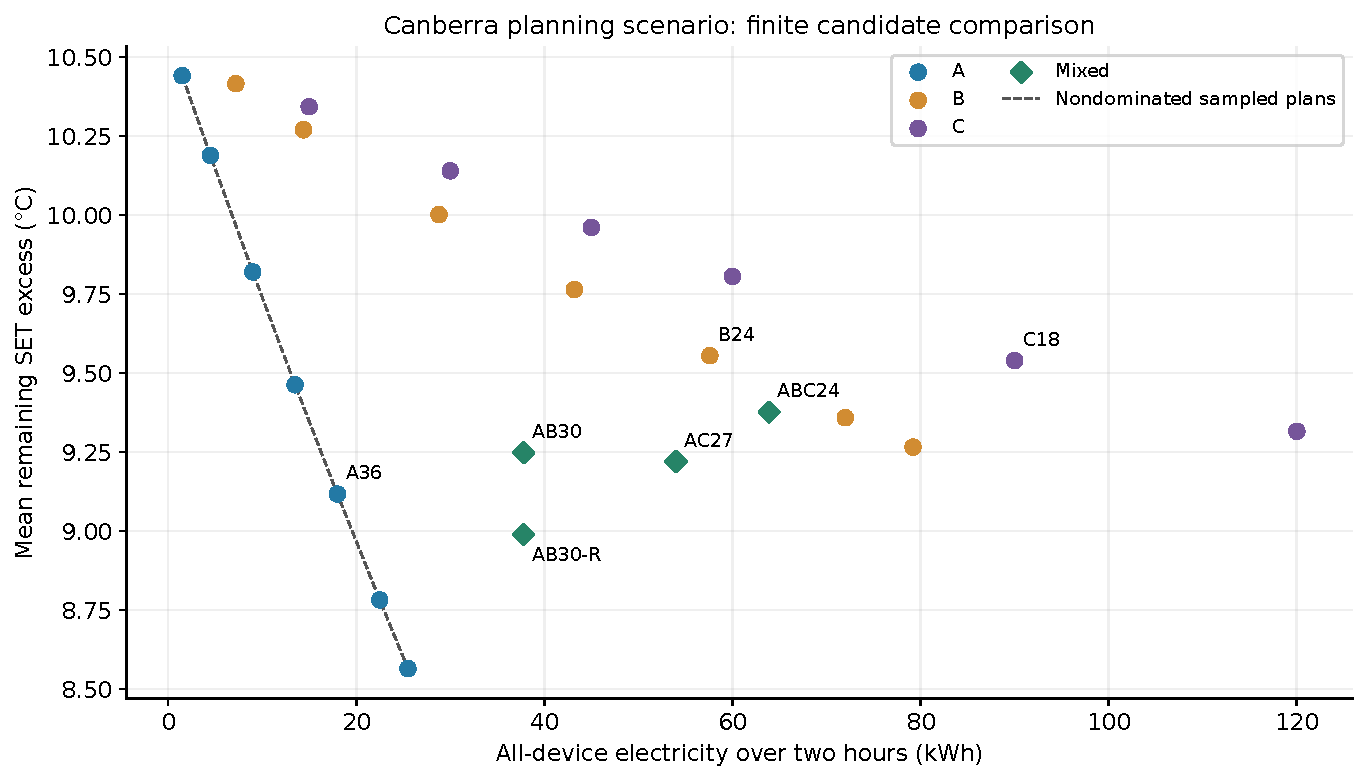
\includegraphics[width=0.90\linewidth]{figures/14_deployment_tradeoff.pdf}
\caption{Energy--discomfort tradeoffs for 24 candidate configurations. The dashed line marks the nondominated candidates; required passenger coverage guides selection.}
\label{fig:deployment-tradeoff}
\end{figure}



\begin{figure}[!ht]
\centering
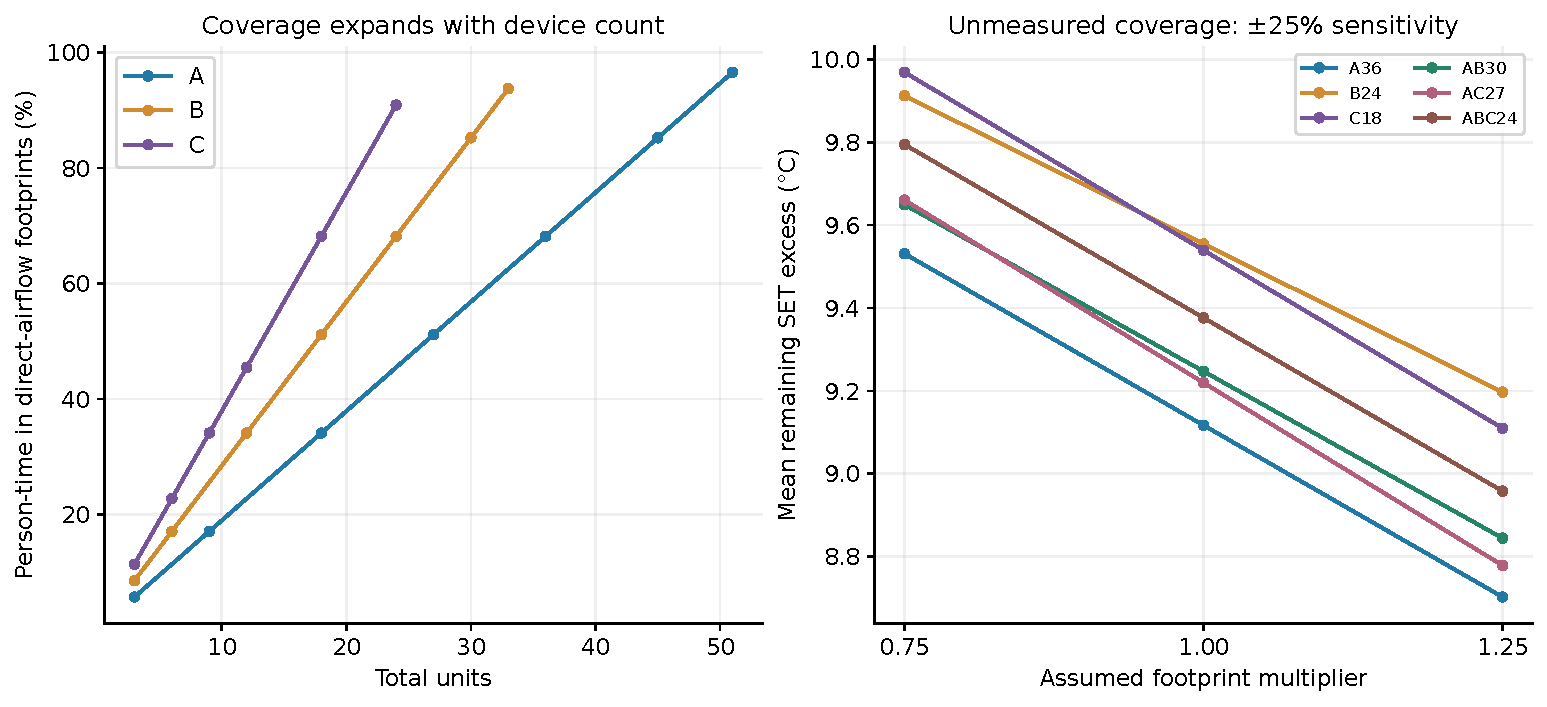
\includegraphics[width=\linewidth]{figures/16_deployment_coverage.pdf}
\caption{Device-count and assumed-footprint sensitivity. Changing footprint affects direct-service fractions; numerical coverage is not a verified equipment rating.}
\label{fig:deployment-coverage}
\end{figure}

\begin{figure}[!ht]
\centering
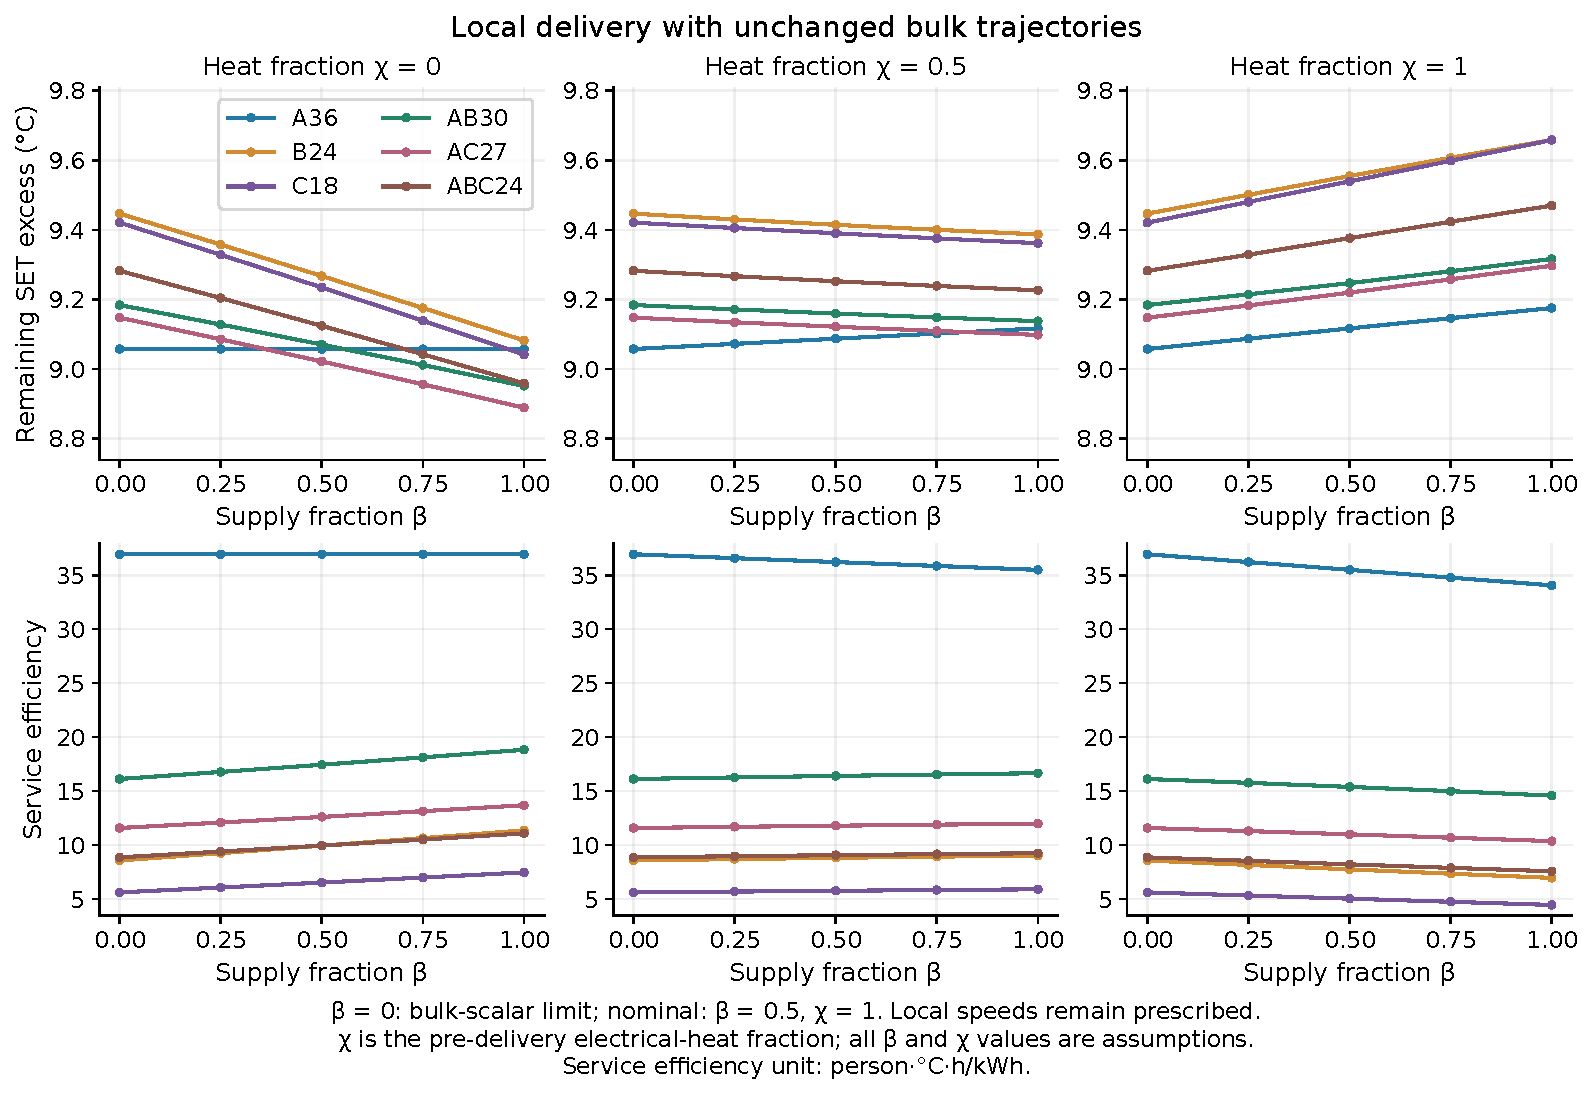
\includegraphics[width=0.96\linewidth]{figures/20_local_delivery_sensitivity.pdf}
\caption{Sensitivity to local stream mixing and supply heat allocation. The parameters are assumptions; $\beta=0$ recovers shared-background exposure. Rankings are conditional on these delivery choices.}
\label{fig:local-sensitivity}
\end{figure}

\subsection{Verification, evidence, and transfer}

The implementation checks both the full background budgets and the local return identities in Eq.~\eqref{eq:return-closure}. Limiting tests recover the old shared-background station calculation at $\beta=0$ and the bus calculation under its fixed-background assumptions. Refining the time step tests integration error; varying $\beta,\chi$ changes local exposure without changing the already balanced background trajectories. The complete check results and trajectories accompany the paper.

\begin{figure}[!ht]
\centering
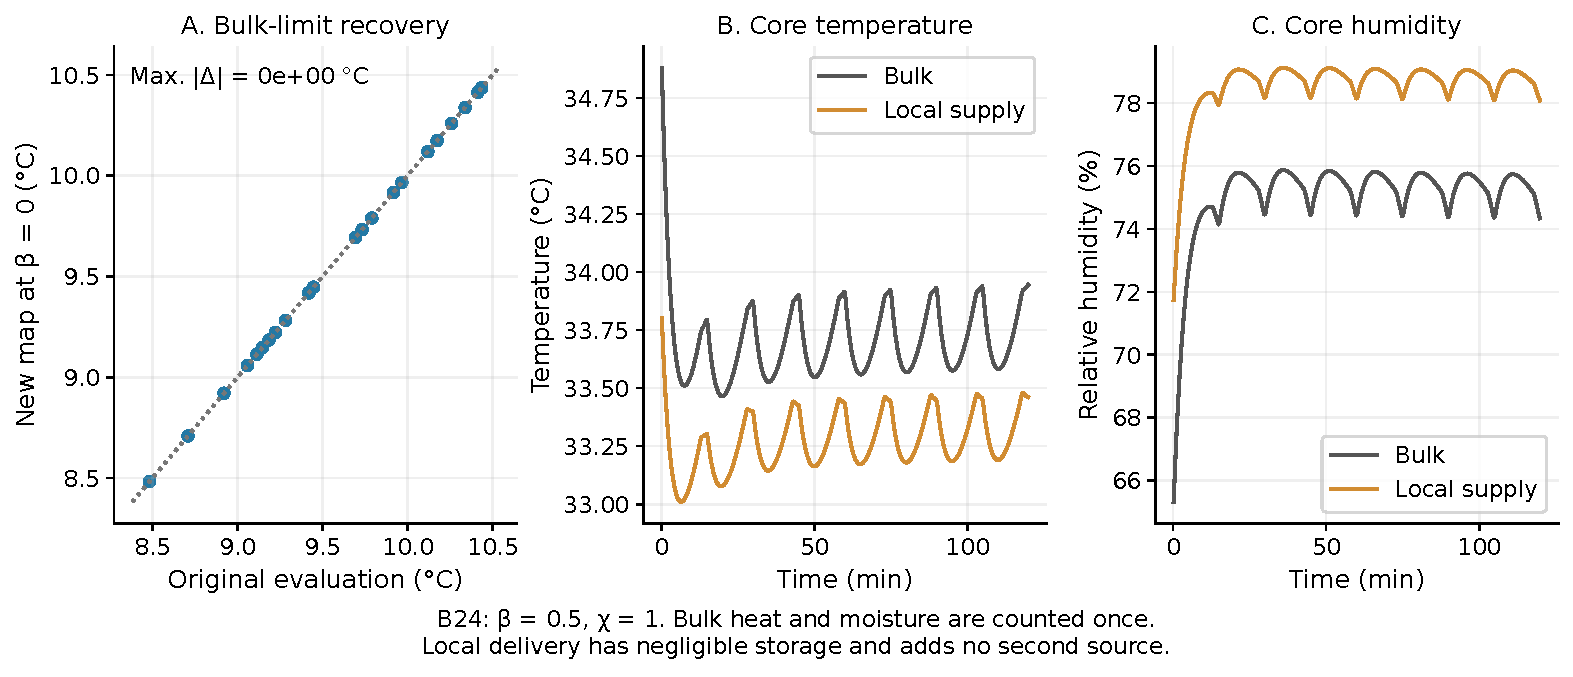
\includegraphics[width=0.92\linewidth]{figures/21_model_reduction_checks.pdf}
\caption{Recovery of the prior station evaluation at $\beta=0$, and local versus background temperature and humidity for B24. Agreement in the limiting case verifies the implementation, not field accuracy.}
\label{fig:reduction-checks}
\end{figure}

The experimental study that informed this structure reports an air-temperature MAE of $0.4\,^{\circ}\mathrm C$ and an RH MAE of about five percentage points for its mist-on validation period \cite{cruz2026}. It separates calibration and validation periods and compares operation against a matched no-mist simulation. We adopt those comparison principles, but its dry-season, unoccupied cafeteria is not a calibration dataset for Canberra. Its reported average $1.9\,^{\circ}\mathrm C$ cooling and mist effectiveness coefficients are not copied into our scenario. It also did not evaluate occupant comfort, so its cooling effectiveness cannot replace our SET-based service measure.

For field validation, first measure the no-device background and estimate exchange and surface response; then measure device outlet and occupied-location $T$, RH and speed to estimate delivery and heat allocation. Use separate periods to test predictions against matched baseline conditions and metered electricity. Compare occupied positions as well as background averages: the study's own well-mixed-zone limitation motivates our local-delivery refinement. Device footprints, passenger distribution, residence times and flows remain uncertain, so present results are conditional comparisons of sampled installations.

The model excludes direct sun, detailed stratification, surface moisture sorption and condensation; it stops on invalid humidity or SET inputs. SET remains quasi-steady even when background conditions evolve. Source code, scenario inputs, numerical checks, CSV outputs and separately replaceable PDF figures are retained in the project. The same chain can be applied to later venues by changing evidenced boundaries and inputs while retaining device, delivery, response and service modules.
